A produção de energia elétrica em Portugal é aberta ao livre mercado e concorrência, tendo dois regimes legais, a saber \cite{REN-site}:
\begin{itemize}
\item Produção em regime ordinário (PRO): relativo à produção de eletricidade a partir de fontes não renováveis ou em grandes centrais hídricas;
\item Produção em regime especial (PRE): relativo à produção de eletricidade a partir de fontes renováveis ou cogeração.
\end{itemize}

O transporte, ou transmissão, da energia elétrica é realizada através da Rede Nacional de Transporte
%\sigla[Rede Nacional de Transporte]{RNT}% 
, a saber a rede de 150 a 400 kV, através de concessão pelo Estado Português em regime de serviço público e exclusividade à Redes Energéticas Nacionais %\sigla[Redes Energéticas Nacionais]{REN}%
. Tal concessão inclui planeamento, construção, operação e manutenção da RNT \cite{REN-site}.

A rede de distribuição é efetivada através da exploração da Rede Nacional de Distribuição %\sigla[Rede Nacional de Distribuição]{RND}%
. A rede de baixa tensão é operada através de contratos estabelecidos entre os municípios e as distribuidoras \cite{REN-site}.

Em relação ao consumo, no Portugal Continental há 6,1 milhões de consumidores em maioria na baixa tensão, 23 500 na média tensão, 350 na alta tensão e muito alta tensão, até 400 kV. O consumidor é livre para escolher o seu comercializador de energia elétrica \cite{REN-site}.

O Sistema Elétrico Nacional %\sigla[Sistema Elétrico Nacional]{SEN}
, ilustrado de forma simplificada na Figura \ref{fig:Organizacao_SEP_PT}, é composto pela parte da produção: PRO, PRE e importação; pela parte do transporte: RNT; pela parte de comercialização: Comercializador Liberalizado e Comercializador de Último Recurso %\sigla[Comercializador de Último Recurso]{CUR}%
; e por fim, pela parcela da distribuição: clientes do mercado liberalizado e do CUR. Os comercializadores liberalizados e de último recurso estão enquadrados no Mercado Organizado. A Entidade Reguladora dos Serviços Energéticos %\sigla[Entidade Reguladora dos Serviços Energéticos]{ERSE}%
é quem estabelece as tarifas pagas pelos comercializadores para acenderem à RNT e RND. Todo esse sistema está sob o enquadramento legislativo e regulamentar da Direção Geral de Energia e Geologia %\sigla[Direção Geral de Energia e Geologia]{DGGE}%
\cite{gil2010analise}.

\begin{figure}[H]
	\centering
	\captionsetup{width=\textwidth, font=footnotesize, textfont=bf}	
	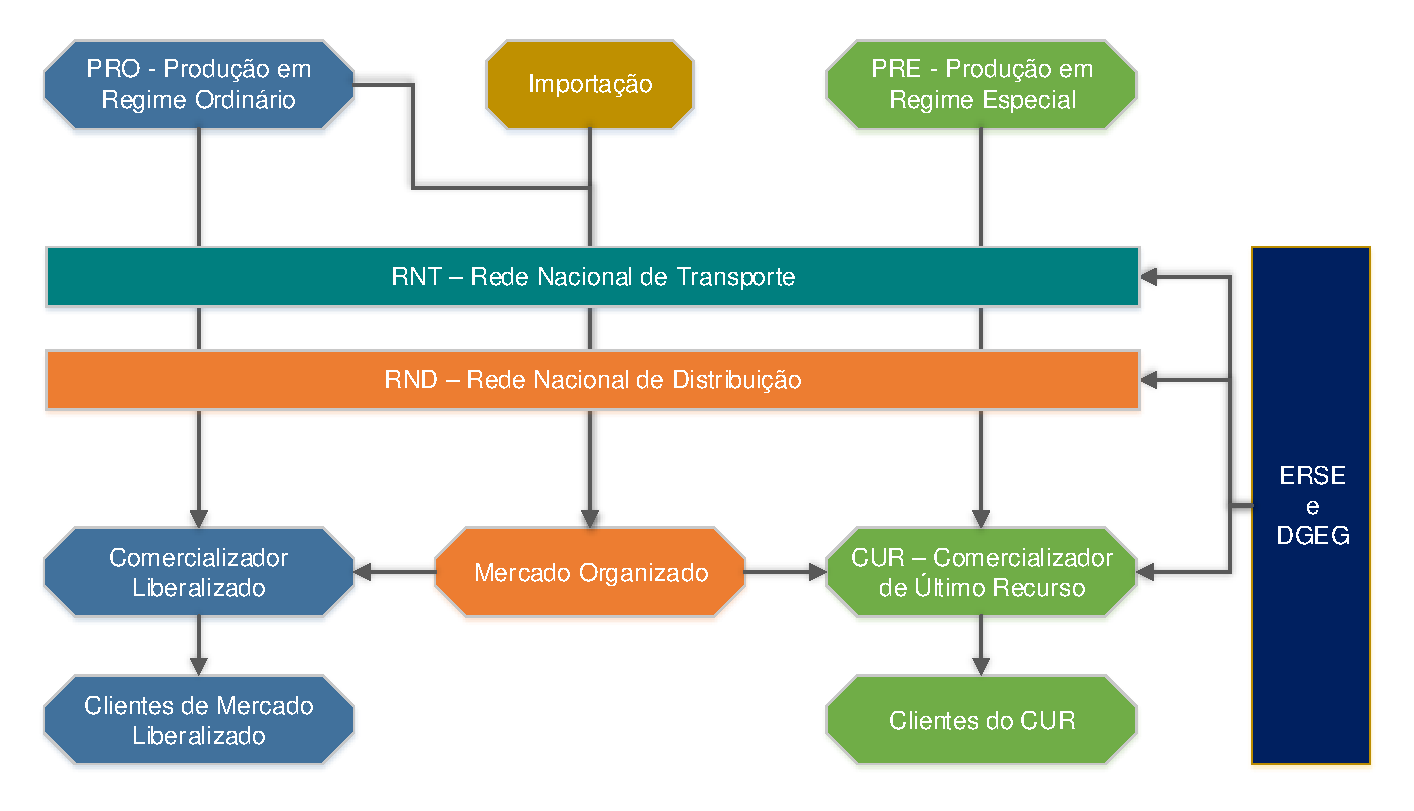
\includegraphics[width=\textwidth]{img/Organizacao_SEP_PT.pdf}
	\caption{Esquema simplificado da Organização do Sistema Elétrico Nacional.}
	\vspace{-3.5mm}
	\caption*{Fonte: \cite{gil2010analise}}
	\label{fig:Organizacao_SEP_PT}
\end{figure}